% Options for packages loaded elsewhere
\PassOptionsToPackage{unicode}{hyperref}
\PassOptionsToPackage{hyphens}{url}
\PassOptionsToPackage{dvipsnames,svgnames,x11names}{xcolor}
%
\documentclass[
  letterpaper,
  DIV=11,
  numbers=noendperiod]{scrartcl}

\usepackage{amsmath,amssymb}
\usepackage{iftex}
\ifPDFTeX
  \usepackage[T1]{fontenc}
  \usepackage[utf8]{inputenc}
  \usepackage{textcomp} % provide euro and other symbols
\else % if luatex or xetex
  \usepackage{unicode-math}
  \defaultfontfeatures{Scale=MatchLowercase}
  \defaultfontfeatures[\rmfamily]{Ligatures=TeX,Scale=1}
\fi
\usepackage{lmodern}
\ifPDFTeX\else  
    % xetex/luatex font selection
  \setmainfont[]{Inter}
  \setsansfont[]{Inter}
  \setmathfont[]{Fira Math}
\fi
% Use upquote if available, for straight quotes in verbatim environments
\IfFileExists{upquote.sty}{\usepackage{upquote}}{}
\IfFileExists{microtype.sty}{% use microtype if available
  \usepackage[]{microtype}
  \UseMicrotypeSet[protrusion]{basicmath} % disable protrusion for tt fonts
}{}
\makeatletter
\@ifundefined{KOMAClassName}{% if non-KOMA class
  \IfFileExists{parskip.sty}{%
    \usepackage{parskip}
  }{% else
    \setlength{\parindent}{0pt}
    \setlength{\parskip}{6pt plus 2pt minus 1pt}}
}{% if KOMA class
  \KOMAoptions{parskip=half}}
\makeatother
\usepackage{xcolor}
\setlength{\emergencystretch}{3em} % prevent overfull lines
\setcounter{secnumdepth}{5}
% Make \paragraph and \subparagraph free-standing
\ifx\paragraph\undefined\else
  \let\oldparagraph\paragraph
  \renewcommand{\paragraph}[1]{\oldparagraph{#1}\mbox{}}
\fi
\ifx\subparagraph\undefined\else
  \let\oldsubparagraph\subparagraph
  \renewcommand{\subparagraph}[1]{\oldsubparagraph{#1}\mbox{}}
\fi


\providecommand{\tightlist}{%
  \setlength{\itemsep}{0pt}\setlength{\parskip}{0pt}}\usepackage{longtable,booktabs,array}
\usepackage{multirow}
\usepackage{calc} % for calculating minipage widths
% Correct order of tables after \paragraph or \subparagraph
\usepackage{etoolbox}
\makeatletter
\patchcmd\longtable{\par}{\if@noskipsec\mbox{}\fi\par}{}{}
\makeatother
% Allow footnotes in longtable head/foot
\IfFileExists{footnotehyper.sty}{\usepackage{footnotehyper}}{\usepackage{footnote}}
\makesavenoteenv{longtable}
\usepackage{graphicx}
\makeatletter
\def\maxwidth{\ifdim\Gin@nat@width>\linewidth\linewidth\else\Gin@nat@width\fi}
\def\maxheight{\ifdim\Gin@nat@height>\textheight\textheight\else\Gin@nat@height\fi}
\makeatother
% Scale images if necessary, so that they will not overflow the page
% margins by default, and it is still possible to overwrite the defaults
% using explicit options in \includegraphics[width, height, ...]{}
\setkeys{Gin}{width=\maxwidth,height=\maxheight,keepaspectratio}
% Set default figure placement to htbp
\makeatletter
\def\fps@figure{htbp}
\makeatother

\usepackage{amsmath, xparse}
\usepackage{fancyvrb, fvextra}
\usepackage{unicode-math}
\usepackage{svg}
\usepackage{multicol}
\usepackage{listings}
\usepackage{systeme}
\usepackage{xifthen}
\DefineVerbatimEnvironment{Highlighting}{Verbatim}{breaklines,commandchars=\\\{\}}
\lstset{basicstyle=\ttfamily\footnotesize,breaklines=true}
\newcommand\rowop[1]{\scriptstyle\smash{\xrightarrow[\vphantom{#1}]{\mkern-4mu#1\mkern-4mu}}}
\DeclareDocumentCommand\converttorows%
{>{\SplitList{,}}m}%
{\ProcessList{#1}{\converttorow}}
\NewDocumentCommand{\converttorow}{m}
{\ifthenelse{\isempty{#1}}{}{\rowop{#1}}\\}

\DeclareDocumentCommand \rowops{m}
{\;
\begin{matrix}
\converttorows {#1}
\end{matrix}
\; }
\KOMAoption{captions}{tableheading}
\makeatletter
\makeatother
\makeatletter
\makeatother
\makeatletter
\@ifpackageloaded{caption}{}{\usepackage{caption}}
\AtBeginDocument{%
\ifdefined\contentsname
  \renewcommand*\contentsname{Table of contents}
\else
  \newcommand\contentsname{Table of contents}
\fi
\ifdefined\listfigurename
  \renewcommand*\listfigurename{List of Figures}
\else
  \newcommand\listfigurename{List of Figures}
\fi
\ifdefined\listtablename
  \renewcommand*\listtablename{List of Tables}
\else
  \newcommand\listtablename{List of Tables}
\fi
\ifdefined\figurename
  \renewcommand*\figurename{Figure}
\else
  \newcommand\figurename{Figure}
\fi
\ifdefined\tablename
  \renewcommand*\tablename{Table}
\else
  \newcommand\tablename{Table}
\fi
}
\@ifpackageloaded{float}{}{\usepackage{float}}
\floatstyle{ruled}
\@ifundefined{c@chapter}{\newfloat{codelisting}{h}{lop}}{\newfloat{codelisting}{h}{lop}[chapter]}
\floatname{codelisting}{Listing}
\newcommand*\listoflistings{\listof{codelisting}{List of Listings}}
\makeatother
\makeatletter
\@ifpackageloaded{caption}{}{\usepackage{caption}}
\@ifpackageloaded{subcaption}{}{\usepackage{subcaption}}
\makeatother
\makeatletter
\@ifpackageloaded{tcolorbox}{}{\usepackage[skins,breakable]{tcolorbox}}
\makeatother
\makeatletter
\@ifundefined{shadecolor}{\definecolor{shadecolor}{rgb}{.97, .97, .97}}
\makeatother
\makeatletter
\makeatother
\makeatletter
\makeatother
\ifLuaTeX
  \usepackage{selnolig}  % disable illegal ligatures
\fi
\IfFileExists{bookmark.sty}{\usepackage{bookmark}}{\usepackage{hyperref}}
\IfFileExists{xurl.sty}{\usepackage{xurl}}{} % add URL line breaks if available
\urlstyle{same} % disable monospaced font for URLs
\hypersetup{
  colorlinks=true,
  linkcolor={blue},
  filecolor={Maroon},
  citecolor={Blue},
  urlcolor={Blue},
  pdfcreator={LaTeX via pandoc}}

\author{}
\date{}

\begin{document}
\begin{titlepage}

    \newcommand{\HRule}{\rule{\linewidth}{0.5mm}}
    
    \center
    
    \vspace{10cm}

    \textsc{\LARGE Gwinnett School of Math, Science, and Technology }\\[0.3cm]
    
    \vspace{0.5cm}

    \HRule \\[0.4cm]
    { \huge \bfseries Macroeconomics Yearlong Notes}\\[0.03cm]
    \HRule \\[1.5cm]
    
    \begin{minipage}{0.4\textwidth}
    \begin{flushleft} \Large
    Anish Goyal \\1st Period
    \end{flushleft}
    \end{minipage}
    ~
    \begin{minipage}{0.4\textwidth}
    \begin{flushright} \Large
    Michael Burbine\\Educator
    \end{flushright}
    \end{minipage}\\[1cm]
    
    {\huge 2023-2024}\\[1cm]
    
    
\includegraphics{img/logo.png}\\
    \vfill
    \end{titlepage}

\newpage

\ifdefined\Shaded\renewenvironment{Shaded}{\begin{tcolorbox}[frame hidden, enhanced, borderline west={3pt}{0pt}{shadecolor}, interior hidden, sharp corners, breakable, boxrule=0pt]}{\end{tcolorbox}}\fi

\renewcommand*\contentsname{Table of Contents}
{
\hypersetup{linkcolor=}
\setcounter{tocdepth}{4}
\tableofcontents
}
\newpage{}

\hypertarget{types-of-goods-0108}{%
\section{Types of Goods (01/08)}\label{types-of-goods-0108}}

\hypertarget{characteristics-of-the-four-types-of-goods}{%
\subsection{Characteristics of the Four Types of
Goods}\label{characteristics-of-the-four-types-of-goods}}

\begin{itemize}
\tightlist
\item
  \textbf{Rivalrous} goods are those that can only be consumed by one
  person at a time.
\item
  \textbf{Non-rivalrous} goods are those that can be consumed by
  multiple people at the same time.
\item
  \textbf{Excludable} goods are those that can be restricted to certain
  people.
\item
  \textbf{Non-excludable} goods are those that cannot be restricted to
  certain people.
\item
  If a public good is overcrowded enough, it can become a common
  resource
\end{itemize}

\hypertarget{the-four-types-of-goods}{%
\subsection{The Four Types of Goods}\label{the-four-types-of-goods}}

\begin{longtable}[]{@{}
  >{\raggedright\arraybackslash}p{(\columnwidth - 2\tabcolsep) * \real{0.1680}}
  >{\raggedright\arraybackslash}p{(\columnwidth - 2\tabcolsep) * \real{0.8320}}@{}}
\toprule\noalign{}
\multicolumn{2}{@{}>{\raggedright\arraybackslash}p{(\columnwidth - 2\tabcolsep) * \real{1.0000} + 2\tabcolsep}@{}}{%
\begin{minipage}[b]{\linewidth}\raggedright
\begin{verbatim}
| **Non-rivalrous** | **Rivalrous** |
\end{verbatim}
\end{minipage}} \\
\midrule\noalign{}
\endhead
\bottomrule\noalign{}
\endlastfoot
\multirow{2}{*}{\textbf{Non-excludable}

==================== \textbf{Excludable}} & \\
& \\
\end{longtable}

\hypertarget{examples}{%
\subsection{Examples}\label{examples}}

\begin{verbatim}
              Case Scenario                   | Type of Good/Service
\end{verbatim}

------------------------------------------------- \textbar{}
-------------------- A college education \textbar{} Artificially scarce
A manicure or pedicure \textbar{} Private good Stone Mountain park
\textbar{} Artificially scarce State park campgrounds \textbar{}
Artificially scarce National defense \textbar{} Public good Peach Pass
lane on I-85 \textbar{} Artificially scarce Fish in the ocean \textbar{}
Common resource Street lights \textbar{} Public good Netflix/Hulu
\textbar{} Artificially scarce Flu shot \textbar{} Private good Tornado
safety shelter \textbar{} Public good Bottled water in a tornado safety
shelter \textbar{} Common resource Hearing a tornado siren \textbar{}
Public good Going to an almost empty public beach \textbar{} Public good
Going to an overcrowded public beach \textbar{} Common resource
St.~Lawrence SeaWay \textbar{} Natural monopoly Flying on a commercial
airplane \textbar{} Natural monopoly Flying a single seat private
airplane \textbar{} Private good Wedding guests eating a slice of the
wedding-cake \textbar{} Common resource Cake sold at a bakery \textbar{}
Private good

\newpage{}

\hypertarget{introduction-to-externalities-0109-0110}{%
\section{Introduction to Externalities
(01/09-01/10)}\label{introduction-to-externalities-0109-0110}}

\hypertarget{overview}{%
\subsection{Overview}\label{overview}}

\begin{itemize}
\tightlist
\item
  An \textbf{externality} is a cost/benefit that affects a \emph{third
  party} who did not choose to incur that cost/benefit.
\item
  They are a type of \textbf{market failure} because they are \emph{not}
  accounted for in the price of the good/service.
\item
  The deadweight loss (DWL) of positive externalities will point to the
  right and vice-versa for negative externalities.

  \begin{itemize}
  \tightlist
  \item
    Which means the DWL triangle always points to the social optimum
    quantity.
  \end{itemize}
\end{itemize}

\hypertarget{internalizing-an-externality-aka-how-to-fix-an-externality}{%
\subsection{\texorpdfstring{Internalizing an Externality (aka \emph{how
to fix an
externality})}{Internalizing an Externality (aka how to fix an externality)}}\label{internalizing-an-externality-aka-how-to-fix-an-externality}}

\hypertarget{problems-with-externalities}{%
\subsubsection{Problems with
externalities}\label{problems-with-externalities}}

\begin{enumerate}
\def\labelenumi{\arabic{enumi})}
\tightlist
\item
  Private individuals won't take into account the external
  costs/benefits
\item
  Public goods and common pool resources tend to lack property rights
\end{enumerate}

\hypertarget{coase-theorem-the-fix}{%
\subsubsection{Coase Theorem (the fix!)}\label{coase-theorem-the-fix}}

``We can fix externalities without the government if we\ldots{}''

\begin{enumerate}
\def\labelenumi{\arabic{enumi})}
\tightlist
\item
  Give property rights to people
\item
  Minimize transaction costs
\end{enumerate}

\hypertarget{examples-1}{%
\subsubsection{Examples}\label{examples-1}}

Methods the government can employ to internalize an externality in a
free market:

\begin{itemize}
\tightlist
\item
  Pollution or emission limits
\item
  ``Pollution credits'' for private firms to buy and sell in the market
\end{itemize}

\newpage{}

\hypertarget{positive-externality-in-consumption}{%
\subsection{Positive Externality in
Consumption}\label{positive-externality-in-consumption}}

\begin{figure}

{\centering 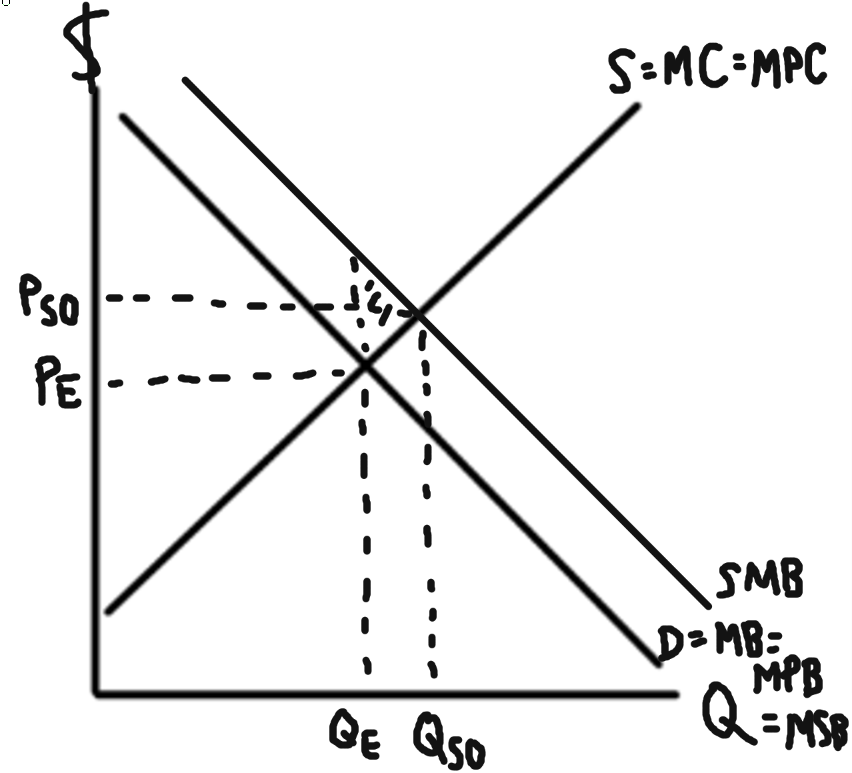
\includegraphics[width=0.5\textwidth,height=\textheight]{img/pos-cons.png}

}

\caption{Positive Externality in Consumption}

\end{figure}

\hypertarget{examples-2}{%
\subsubsection{Examples}\label{examples-2}}

\begin{itemize}
\tightlist
\item
  Consumption of education
\item
  Consumption of health care
\item
  Advertisement can lead to an increase of demand in the free market
  \(\therefore MPB\) goes up and moves the market toward \(MSB\).
\end{itemize}

\hypertarget{spillover-effect}{%
\subsubsection{Spillover Effect}\label{spillover-effect}}

\begin{itemize}
\tightlist
\item
  The spillover effect is \(MEB = MSB-MPB\).
\item
  \(MPB < MSB\)
\item
  \(MPC = MSC\)
\end{itemize}

\hypertarget{internalizing-the-spillover-effect}{%
\subsubsection{Internalizing the Spillover
Effect}\label{internalizing-the-spillover-effect}}

\begin{itemize}
\tightlist
\item
  The external \textbf{benefits} can be internalized by
  \textbf{subsidizing} the product/service to the consumers of the
  good/service.
\item
  The government intervention will move the private market to
  \textbf{social optimum} where \(MSB = MSC\).
\end{itemize}

\newpage{}

\hypertarget{negative-externality-in-consumption}{%
\subsection{Negative Externality in
Consumption}\label{negative-externality-in-consumption}}

\begin{figure}

{\centering 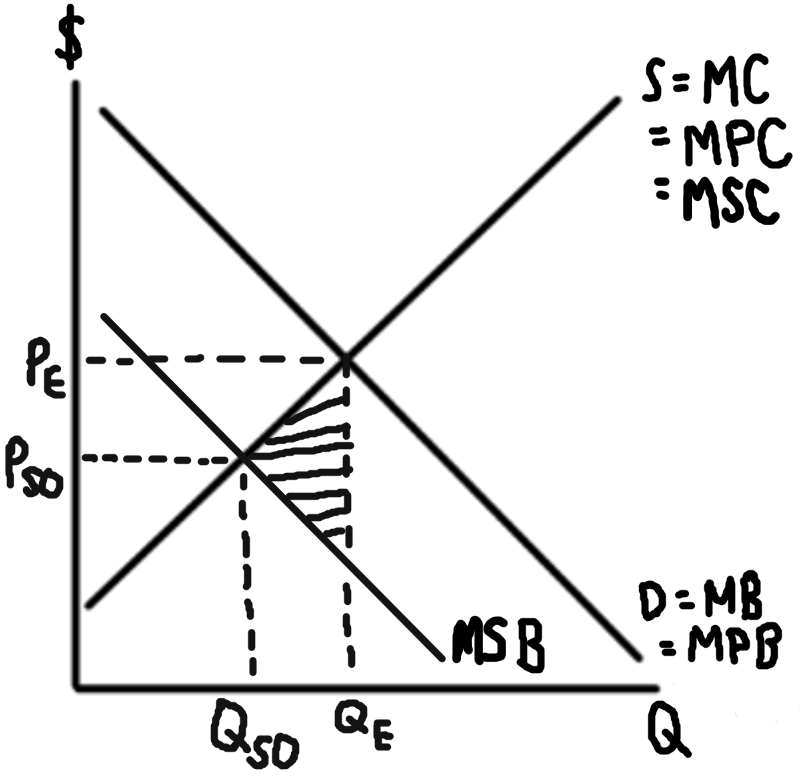
\includegraphics[width=0.45\textwidth,height=\textheight]{img/neg-cons.png}

}

\caption{Negative Externality in Consumption}

\end{figure}

\hypertarget{examples-3}{%
\subsubsection{Examples}\label{examples-3}}

\begin{itemize}
\tightlist
\item
  Smoking in public/passive smoking
\item
  Pollution due to fossil fuels
\item
  Playing loud music
\item
  Discarding garbage in public places
\end{itemize}

\hypertarget{spillover-effect-1}{%
\subsubsection{Spillover Effect}\label{spillover-effect-1}}

\begin{itemize}
\tightlist
\item
  The spillover effect is \(MEB = MSB-MPB\).
\item
  \(MPB > MSB\)
\item
  \(MPC = MSC\)
\end{itemize}

\hypertarget{internalizing-the-spillover-effect-1}{%
\subsubsection{Internalizing the Spillover
Effect}\label{internalizing-the-spillover-effect-1}}

\begin{itemize}
\tightlist
\item
  The external \textbf{benefits} can be internalized by \textbf{imposing
  a tax} on the product/service to the consumers of the good/service.
\item
  The government intervention will move the private market to
  \textbf{social optimum} where \(MSB = MSC\).
\end{itemize}

\newpage{}

\hypertarget{positive-externality-in-production}{%
\subsection{Positive Externality in
Production}\label{positive-externality-in-production}}

\begin{figure}

{\centering 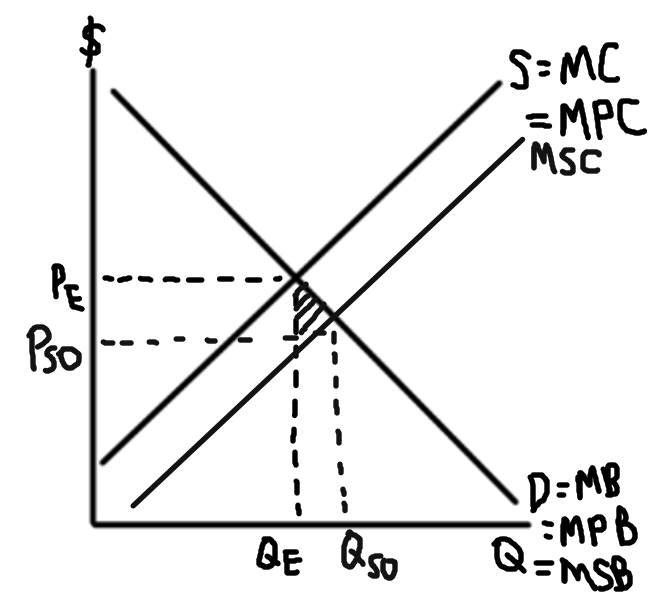
\includegraphics[width=0.5\textwidth,height=\textheight]{img/pos-prod.png}

}

\caption{Positive Externality in Production}

\end{figure}

\hypertarget{examples-4}{%
\subsubsection{Examples}\label{examples-4}}

\begin{itemize}
\tightlist
\item
  Companies invest in training/professional development of their
  employees.
\item
  Firms invest in research and development (R\&D).
\end{itemize}

\hypertarget{spillover-effect-2}{%
\subsubsection{Spillover Effect}\label{spillover-effect-2}}

\begin{itemize}
\tightlist
\item
  The spillover effect is \(MEC = MSC-MPC\).
\item
  \(MPB = MSB\)
\item
  \(MPC > MSC\)
\end{itemize}

\hypertarget{internalizing-the-spillover-effect-2}{%
\subsubsection{Internalizing the Spillover
Effect}\label{internalizing-the-spillover-effect-2}}

\begin{itemize}
\tightlist
\item
  The external \textbf{costs} can be internalized by
  \textbf{subsidizing} the product/service to the producers of the
  good/service.
\item
  The government intervention will move the private market to
  \textbf{social optimum} where \(MSB = MSC\).
\end{itemize}

\newpage{}

\hypertarget{negative-externality-in-production}{%
\subsection{Negative Externality in
Production}\label{negative-externality-in-production}}

\begin{figure}

{\centering 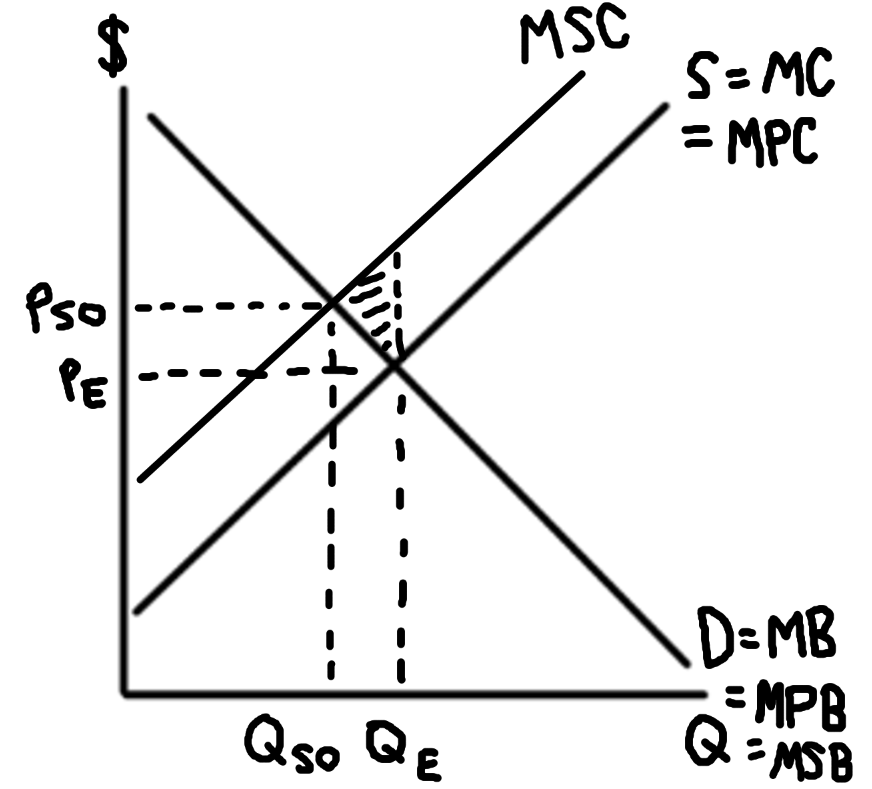
\includegraphics[width=0.5\textwidth,height=\textheight]{img/neg-prod.png}

}

\caption{Negative Externality in Production}

\end{figure}

\hypertarget{examples-5}{%
\subsubsection{Examples}\label{examples-5}}

\begin{itemize}
\tightlist
\item
  Firms produce chemicals that cause pollution \(\therefore\) local
  fisherman cannot catch fish.
\item
  Construction of roads lead to change of landscape and parks
\item
  Coal fired power plants
\end{itemize}

\hypertarget{spillover-effect-3}{%
\subsubsection{Spillover Effect}\label{spillover-effect-3}}

\begin{itemize}
\tightlist
\item
  The spillover effect is \(MEC = MSC-MPC\).
\item
  \(MPB = MSB\)
\item
  \(MPC < MSC\)
\end{itemize}

\hypertarget{internalizing-the-spillover-effect-3}{%
\subsubsection{Internalizing the Spillover
Effect}\label{internalizing-the-spillover-effect-3}}

\begin{itemize}
\tightlist
\item
  The external \textbf{costs} can be internalized by \textbf{imposing a
  tax} on the product/service to the producers of the good/service.
\item
  The government intervention will move the private market to
  \textbf{social optimum} where \(MSB = MSC\).
\end{itemize}

\newpage{}

\hypertarget{income-inequality-0112}{%
\section{Income Inequality (01/12)}\label{income-inequality-0112}}

\hypertarget{the-lorenz-curve-and-gini-coefficient}{%
\subsection{The Lorenz Curve and Gini
Coefficient}\label{the-lorenz-curve-and-gini-coefficient}}

\begin{itemize}
\tightlist
\item
  The \textbf{Lorenz Curve} \(L(x)\) is a graphical representation of
  the distribution of income in a country.

  \begin{itemize}
  \tightlist
  \item
    The x-axis is the cumulative percentage of the population
    (0\%-100\%).
  \item
    The y-axis is the cumulative percentage of income (0\%-100\%).
  \item
    It is always accompanied by the line \(y=x\) which represents
    \textbf{perfect equality}.
  \end{itemize}
\item
  The \textbf{Gini Coefficient} \(G\) is a numerical representation of
  the Lorenz Curve.

  \begin{itemize}
  \tightlist
  \item
    It is the ratio of the area between the Lorenz Curve and the line
    \(y=x\) to the area under the line \(y=x\).

    \begin{itemize}
    \tightlist
    \item
      \(G = \frac{A}{A+B}\) where
      \(A = \int_{0}^{1} \left[x-L(x)\right] \ \mathrm{d}x\) and
      \(B = \int_{0}^{1}L(x) \ \mathrm{d}x\).
    \end{itemize}
  \item
    The closer \(G\) is to 1, the more unequal the distribution of
    income is.
  \end{itemize}
\end{itemize}

\begin{figure}

{\centering 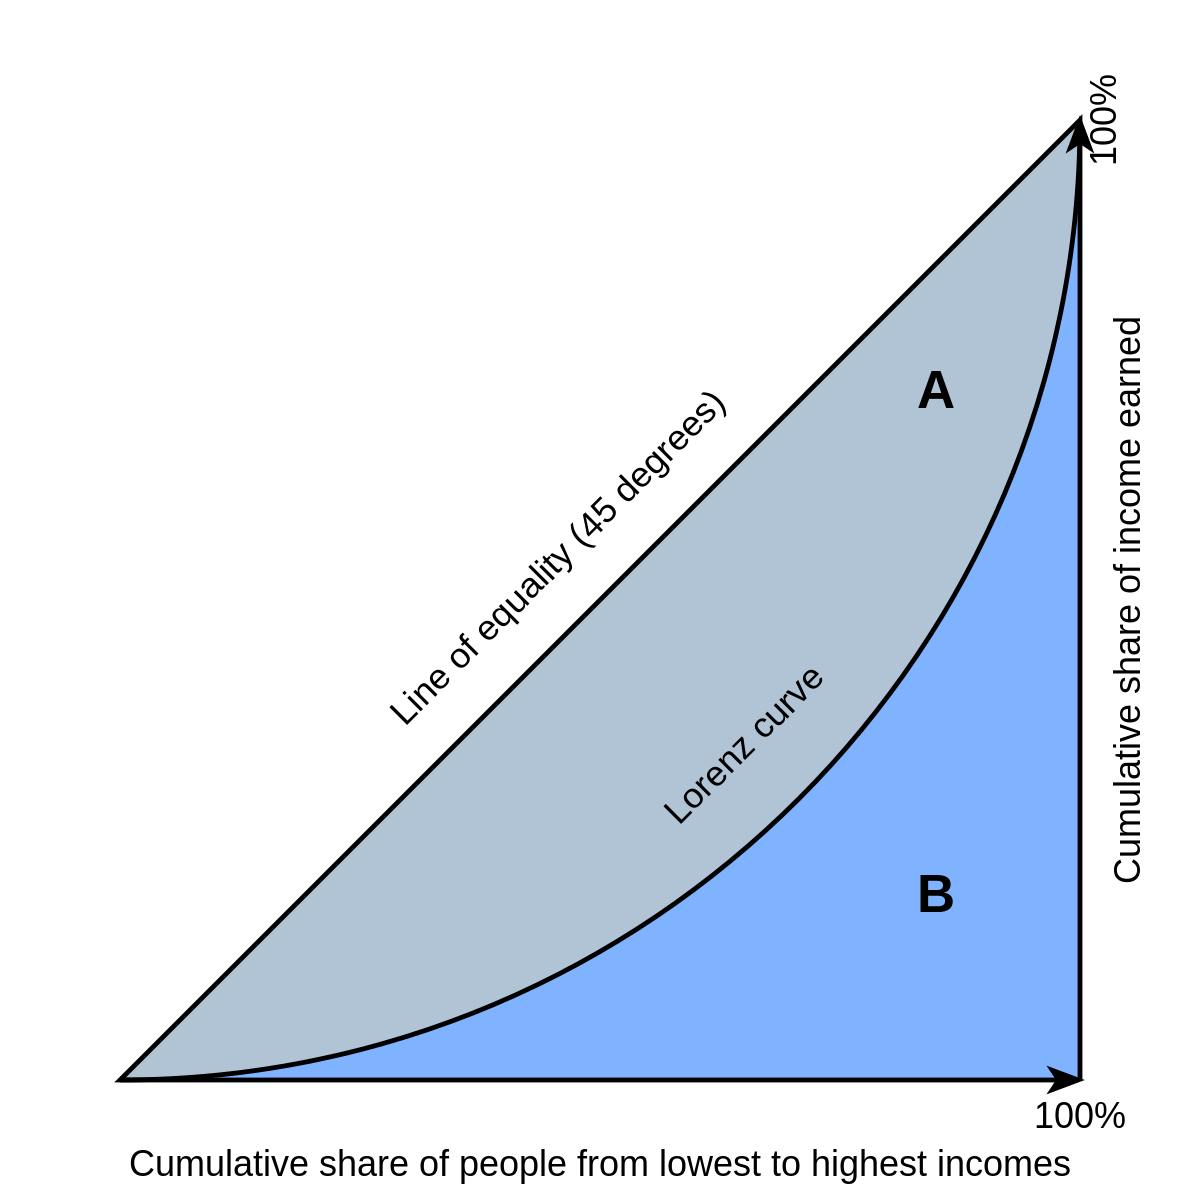
\includegraphics[width=0.68\textwidth,height=\textheight]{img/lorenz.png}

}

\caption{Visual depiction of the Lorenz Curve}

\end{figure}

As demonstrated in \emph{Figure 6} below:

\begin{itemize}
\tightlist
\item
  If \(G\) is 0, then the Lorenz Curve is \textbf{also} the line \(y=x\)
  because the area between both curves \(A\) is 0.
\item
  If \(G\) is 1, then the Lorenz Curve is the x-axis (\(y=0\)) because
  \(A+B\) must also equal the area under \(y=x\), or \(\frac{1}{2}\).
\end{itemize}

\begin{figure}

{\centering 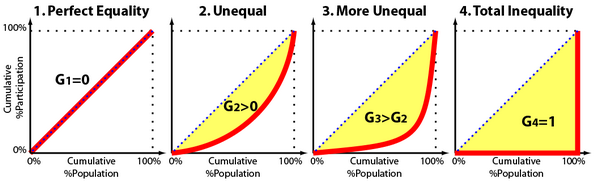
\includegraphics[width=1\textwidth,height=\textheight]{img/varying-gini.png}

}

\caption{Varying Gini Coefficients and their corresponding Lorenz
Curves}

\end{figure}

\hypertarget{deriving-simpler-expressions-for-the-gini-coefficient}{%
\subsection{Deriving Simpler Expressions for the Gini
Coefficient}\label{deriving-simpler-expressions-for-the-gini-coefficient}}

Since we know that
\(A+B = \int_{0}^{1} x \ \mathrm{d}x = \left.\frac{x^2}{2}\right\vert_{0}^{1} = \frac{1}{2}\),
we can derive ``easier'' expressions to calculate the Gini Coefficient
\(G\).

\hypertarget{deriving-g2a}{%
\subsubsection{\texorpdfstring{Deriving
\(G=2A\)}{Deriving G=2A}}\label{deriving-g2a}}

\begin{align}
G &= \frac{A}{A+B}\tag{Initial Gini Coefficient formula} \\
\frac{1}{G} &= \frac{A+B}{A}\tag{Reciprocate} \\
\frac{A}{G} &= A+B\tag{Multiply by $A$} \\
\frac{A}{G}-A &= B\tag{Subtract $A$}
\end{align}

\newpage{}

Now we can substitute \(B\) into the original area formula:

\begin{align}
A + B &= \frac{1}{2}\tag{Area under $y=x$} \\
A+\left(\frac{A}{G}-A\right) &= \frac{1}{2}\tag{Substitute $B$} \\
\frac{A}{G} &= \frac{1}{2}\tag{Simplify} \\
\cfrac{A}{\frac{1}{2}} &= G\tag{Simplify} \\
2A &= G\tag{Multiply by 2}
\end{align}

\hypertarget{deriving-g1-2b}{%
\subsubsection{\texorpdfstring{Deriving
\(G=1-2B\)}{Deriving G=1-2B}}\label{deriving-g1-2b}}

Since we've already expressed \(B\) in terms of \(A\), we just need to
get \(A\) in terms of \(B\).

\begin{align}
G = 2A \tag{Previous derivation} \\
\frac{G}{2} = A \tag{Divide by 2} \\
\frac{G}{2} = \frac{1}{2}-B\tag{Substitute $A$ using the expression $A=\frac{1}{2}-B$} \\
G = 1-2B\tag{Multiply by 2}
\end{align}

Therefore, two \textbf{alternate expressions} for the Gini Coefficient
are:

\begin{align}
G &= 2A \\
G &= 1-2B
\end{align}

\newpage{}

\hypertarget{negative-externalities-public-vs.-private-resolution-and-more-on-the-coase-theorem-0116}{%
\subsection{Negative Externalities: Public vs.~Private Resolution and
More on the Coase Theorem
(01/16)}\label{negative-externalities-public-vs.-private-resolution-and-more-on-the-coase-theorem-0116}}

For each of the following case scenarios, indicate how plausible it is
for the stakeholders to mitigate the effects of a negative externality
through private negotiation.

\hypertarget{conditions}{%
\subsubsection{Conditions}\label{conditions}}

\begin{itemize}
\tightlist
\item
  Both sides are rational and willing to negotiate tomaximize their own
  utility.
\item
  Low to no transaction cost
\item
  Private property rights are well defined
\item
  Perfect information is available to both sides and they have the same
  leverage
\end{itemize}

\begin{longtable}[]{@{}
  >{\raggedright\arraybackslash}p{(\columnwidth - 0\tabcolsep) * \real{1.0044}}@{}}
\toprule\noalign{}
\begin{minipage}[b]{\linewidth}\raggedright
\textbf{Scenario} \textbar{} \textbf{Private resolution is} ~\textbar{}
\textbf{Private resolution seems} ~\textbar{} \textbf{Private resolution
is very} ~\textbar{} \textbar{} \textbf{very unlikely} \textbar{}
\textbf{possible} \textbar{} \textbf{likely} \textbar{}
====================+:==========================================================+:==========================================+
\textbf{Non-excludable} \textbar{} \emph{Public Goods}~ \textbar{}
\emph{Common-Pool/Common Resources}~ \textbar{} \textbar{} (e.g.~Sunset,
Common Knowledge) \textbar{} (e.g.~Irrigation Systems, Libraries)
\textbar{}
====================+=============================================================+======================================+
\textbf{Excludable} \textbar{} \emph{(Toll/Club/Artificially Scarce)
Goods/Natural monopolies}~\textbar{} \emph{Private Goods}~ \textbar{}
\textbar{} (e.g.~Day-Care Centers, Country Clubs) \textbar{}
(e.g.~Donuts, Personal Computers) \textbar{}
\end{minipage} \\
\begin{minipage}[b]{\linewidth}\raggedright
====================+:==========================================================+:==========================================+
\textbf{Non-excludable} \textbar{} \emph{Public Goods}~ \textbar{}
\emph{Common-Pool/Common Resources}\\
\textbar{} (e.g.~Sunset, Common Knowledge) \textbar{} (e.g.~Irrigation
Systems, Libraries)\strut
\end{minipage} \\
\midrule\noalign{}
\endhead
\bottomrule\noalign{}
\endlastfoot
\end{longtable}



\end{document}
